\chapter{Anhang}
\section{Exposé}
Das Exposé wurde zu Beginn der Arbeit verfasst und legt Motivation und Problemstellung dar. Weiterhin werden der Fokus der Arbeit sowie die Herangehensweise skizziert. Es wurde im Rahmen der Anmeldung beim Prüfungsamt als verbindliche Aufgabenstellung beigelegt. 
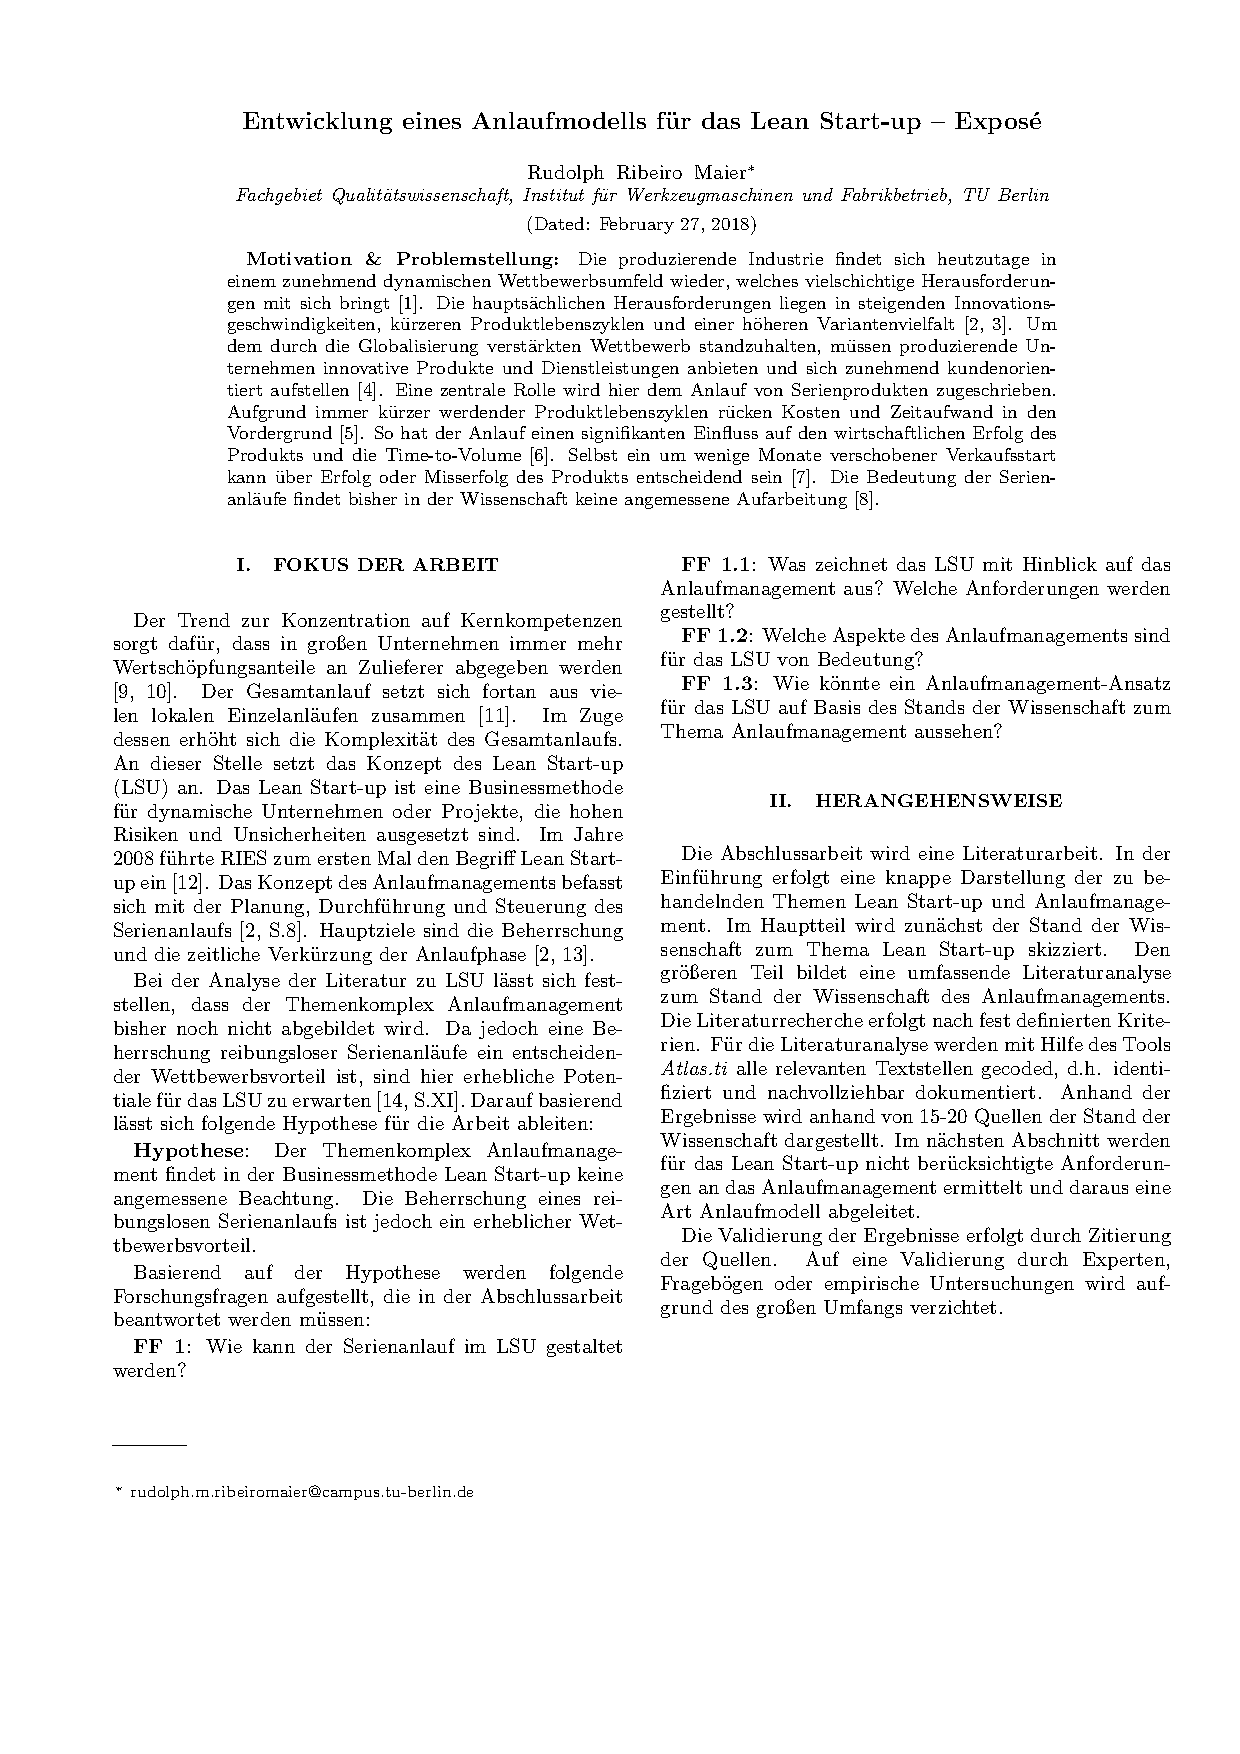
\includepdf[pages={1,2}]{latex_settings/onepager.pdf}			% Aufgabenstellung

% \chapter{Ergänzungen}
\newgeometry{left=30mm, right=30mm, top=20mm, bottom=5mm}
\section{Die Entwicklung des Grundgerüsts}
\begin{figure}[ht]
 \centering
 \includegraphics[scale=.76,clip=true,trim=30 50 30 40]{./img/Kollage.pdf}
 % Kollage.pdf: 0x0 pixel, 300dpi, 0.00x0.00 cm, bb=
 \caption{Entwicklung des Grundgerüsts}
 \label{fig:kollage}
\end{figure}

\clearpage
\restoregeometry

\section{Dombrowski-2011a - Lean Ramp-up. Handlungs- und Gestaltungsfelder}
\subsection*{Die Handlungsfelder im Lean Ramp-up}\label{appendix:dom11a:hf}
\begin{description}

\item[Produktentwicklung und Konstruktion]
umfassen alle Aufgaben, die sich mit
dem Konzipieren, Entwerfen, Ausarbeiten und Erproben eines Produkts
beschäftigen. Als Ergebnis resultieren Zeichnungen, Stücklisten und andere Produktdokumentationen.

\item[Fertigungs- und Montagemittel] umfassen alle Aufgaben, die sich mit der Bedarfsplanung, Auswahl, Beschaffung,
Herstellung, Einrichtung, Programmierung und Inbetriebnahme von Maschinen, Anlagen, Werkzeugen und
Vorrichtungen beschäftigen. Dazu gehören auch die Wartung und Instandhaltung. Als Ergebnis resultiert ein
Fertigungs- und Montagekonzept.

\item[Fertigungs- und Montageprozesse] umfassen alle Aufgaben, die sich mit der
Festlegung der Arbeitsabläufe zur
Herstellung eines Produkts in der
Fertigung und Montage beschäftigen.
Es werden u. a. Reihenfolgen und
Vorgabezeiten bestimmt sowie Produktionsmittel zugeordnet. Als Ergebnis resultieren Arbeitspläne, in
denen alle Informationen dokumentiert sind.

\item[Personal- und Arbeitsorganisation] umfasst alle Aufgaben, die sich mit der
Bedarfs- und Einsatzplanung, Beschaffung, Entwicklung und Freisetzung von Personal sowie mit der Gestaltung einer arbeitsgerechten und
bestmöglichen Zusammenarbeit von
Mensch und Technik beschäftigen.
Als Ergebnis resultieren zum Beispiel
Personaleinsatzpläne,
 Arbeitszeitund Entgeltsysteme.

\item[Produktionsplanung und -steuerung]
(PPS) umfasst alle Aufgaben, die sich
mit der Festlegung, Veranlassung,
Überwachung und Sicherung des Produktionsprogramms nach Art und
Menge unter Berücksichtigung von
Terminen und Kapazitäten beschäftigen. Als Ergebnis resultiert ein Produktionsplan mit Bedarfsmengen und
-terminen für Zukauf- und Eigenfertigungsteile.

 \item[Einkaufs- und Dispositionsprozesse]
umfassen alle Aufgaben, die sich mit
der kostenoptimalen strategischen
und operativen Beschaffung von Zukaufteilen, Handelswaren, Betriebsmitteln und Dienstleistungen von einem Lieferanten beschäftigen. Als Ergebnis resultieren zum Beispiel Sourcingstrategien, Verträge mit Lieferanten und verfügbare Lagerbestände.


 \item[Logistikprozesse und Logistikmittel]
umfassen alle Aufgaben, die sich mit
der Festlegung von effizienten inner-
und außerbetrieblichen Transporten
bzw. Materialflüssen und der Bereitstellung von Gütern beschäftigen.
Außerdem werden Logistikmittel, wie
z. B. Lager- und Transportmittel bestimmt. Als Ergebnis resultieren sog.
Logistiksysteme.

 \item[Gebäude, Layout und Arbeitsplätze]
umfassen alle fabrikplanerischen Aufgaben, die sich mit der Festlegung, optimalen Auslegung und Realisierung
der Produktionsstätten beschäftigen.
Der Umfang reicht dabei von der Umgestaltung einzelner Arbeitsplätze bis
hin zur Errichtung neuer Gebäude.
Als Ergebnis resultieren eingerichtete
Arbeitsplätze, Flächen und Gebäude.


 \item[Qualitätsmanagement und Qualitätsmittel] umfassen alle Aufgaben, die
sich mit der Planung, Lenkung, Prüfung, Sicherung und Verbesserung
der Qualitätsmerkmale von Produkten, Prozessen und Leistungen beschäftigen. Außerdem werden Qualitätsmittel, wie z. B. Prüf- und Messmittel bestimmt. Als Ergebnis resultieren beispielsweise Arbeits- und
Prüfanweisungen.

\item[Informationsprozesse und -systeme]
umfassen alle Aufgaben, die sich mit
der Beschaffung, Verarbeitung, Übertragung und Speicherung von Informationen zur Integration und zielorientierten Steuerung aller operativen Prozesse beschäftigen. Als Ergebnis resultieren zum Beispiel Systeme
zur Betriebsdatenerfassung (BDE).
\end{description}

\subsection*{Die Gestaltungsfelder im Lean Ramp-up}\label{appendix:dom11a:gf}
\begin{description}
\item[Integration und Kooperation] umfassen
alle Methoden und Werkzeuge, die
fachbereichs-, pha\-sen"~, technologie- und unternehmensübergreifend zur
Synchronisierung von Produkt- und
Produktionsentwicklung beitragen.
Dazu wird eine simultane, interdisziplinäre und partnerschaftliche Zusammenarbeit angestrebt. Ziel ist es,
zum Beispiel Schnittstellen und Änderungen zu reduzieren.

\item[Partizipation und Veränderung] umfassen alle Methoden und Werkzeuge,
die zur Motivation der Mitarbeiter
und zum Abbau bzw. zur Vermeidung
von Widerständen und Konflikten beitragen. Dazu werden alle betroffenen
Organisationseinheiten am ProdukBild 4. Gestaltungsfelder im Lean Ramp-up
tionsanlauf beteiligt. Ziel ist es, die
Potenziale der Mitarbeiter zu nutzen
und einen reibungslosen Anlauf zu erreichen.

 \item[Wertschöpfung und Just-in-Time (JIT)]
umfassen alle Methoden und Werkzeuge, die zur produktiven, schnellen
und termingerechten Herstellung
bzw. Lieferung der Produkte beitragen. Dazu werden alle Verluste in den
Produktions- und Logistikprozessen
eliminiert und eine fließende und
kundenorientierte Produktion aufgebaut. Ziel ist ein schlankes Produktionssystem.

 \item[Pilotierung und Qualifizierung] umfasst
alle Methoden und Werkzeuge, die
zur Absicherung von Produkt- und
Prozessreifegrad sowie zur Steigerung der Leistungsfähigkeit des Produktionssystems beitragen. Dazu
werden sog. Pilotbereiche eingerichtet in denen Produktionstests sowie
Mitarbeiterschulungen erfolgen. Ziel
ist eine steile Lern- bzw. Anlaufkurve.

 \item[Priorisierung und Standardisierung]
umfassen alle Methoden und Werkzeuge, die zur Reduzierung, Beherrschung und Vermeidung der technologischen, prozessualen und organisatorischen Komplexität im Produktionsanlauf beitragen. Dazu werden
Schwerpunkte gebildet und Referenzunterlagen erstellt. Ziel ist es, den
Aufwand im Produktionsanlauf zu reduzieren.

 \item[Reaktionsfähigkeit und Flexibilität] umfassen alle Methoden und Werkzeuge,
die zum zeitnahen Erkennen veränderter Randbedingungen und Störungen sowie zur kontinuierlichen Anpassung des Anlaufmanagements beitragen. Dazu werden Frühwarnsysteme etabliert und Handlungsoptionen
bestimmt. Ziel ist es, schnell auf Veränderungen und Störungen zu reagieren.

 \item[Fehler- und Risikovermeidung] umfasst
alle Methoden und Werkzeuge, die
zur präventiven Qualitätssicherung
und -verbesserung beitragen. Dazu
werden frühzeitig die Ergebnisse der
Produkt- und Produktionsentwicklung veranschaulicht und Fehler- bzw.
Risikopotentiale eliminiert. Ziel sind
eine hohe Produkt- und Prozessqualität sowie geringe Änderungs- und
Prüfkosten.

 \item[Problemlösung und Stabilisierung] umfassen alle Methoden und Werkzeuge,
die zur reaktiven Qualitätssicherung
und -verbesserung beitragen. Dazu
werden die Produkte und Prozesse
kontinuierlich überprüft und überwacht sowie systematisch Problemursachen beseitigt. Ziel ist eine Stabilisierung des Anlaufs und Vermeidung
von Folge- und Wiederholungsfehlern.

 \item[Wissenstransfer und KVP] umfassen
alle Methoden und Werkzeuge, die
zum Transfer von Erfahrungswissen
und zur Erhöhung der Mitarbeiterkompetenzen beitragen. Dazu wird
explizites und – soweit möglich – implizites Wissen identifiziert, gesammelt, aufbereitet und vermittelt. Ziel
ist es, mit dessen Nutzung und
Weiterentwicklung aktuelle und zukünftige Anläufe zu verbessern.

 \item[Transparenz und Visualisierung] umfassen alle Methoden und Werkzeuge,
die zur Verfügbarkeit und leicht verständlichen Darstellung von Informationen und Daten beitragen. Dazu
werden sowohl informations- und
kommunikationstechnische Systeme
als auch optische Hilfsmittel und Signale eingesetzt. Ziel ist die Regelung,
Steuerung und Verbesserung des Produktionsanlaufs.
\end{description}


\newpage
%   left=30mm, right=30mm, top=20mm, bottom=20mm, % margins

\newgeometry{left=30mm, right=30mm, top=20mm, bottom=5mm}
\section{Dombrowski-2011b - Lean Ramp-up: Schwerpunkte im Anlaufmanagement}
\begin{figure}[h!]
 \centering
 \includegraphics[scale=.3]{./img/dom11b:firstmover.png}
 % dom11b:firstmover.png: 0x0 pixel, 0dpi, 0.00x0.00 cm, bb=
 \caption[Schwerpunkte für \textit{Firstmover}]{Schwerpunkte für \textit{Firstmover} \autocite{Dombrowski2011b}}
 \label{fig:dom11b:firstmover}
 \vspace{8mm}
% \end{figure}
% 
% 
% \begin{figure}[h]
 \centering
 \includegraphics[scale=.3]{./img/dom11b:kostenfuehrer.png}
 % dom11b:firstmover.png: 0x0 pixel, 0dpi, 0.00x0.00 cm, bb=
 \caption[Schwerpunkte für \textit{Follower (Kosten)}]{Schwerpunkte für \textit{Follower (Kosten)} \autocite{Dombrowski2011b}}
 \label{fig:dom11b:kostenfuehrer}
 \vspace{8mm}
% \end{figure}
% 
% 
% \begin{figure}[h]
 \centering
 \includegraphics[scale=.3]{./img/dom11b:qualitaetsfuehrer.png}
 % dom11b:firstmover.png: 0x0 pixel, 0dpi, 0.00x0.00 cm, bb=
 \caption[Schwerpunkte für \textit{Follower (Qualität)}]{Schwerpunkte für \textit{Follower (Qualität)} \autocite{Dombrowski2011b}}
 \label{fig:dom11b:qualitaetsfuehrer}
%  \vspace{5mm}
\end{figure}
\restoregeometry